% =============================================================================
% sections/design/drone/navigation_perception.tex  -  Navigation and Perception
% Teams: drone (best guess - unconfirmed) / Status: EXAMPLE (scope approximation)
%
% EXAMPLE CONTENT for scope/layout approximation - not final report text.
% Adapted from the Preliminary Report's "Autonomous Navigation Pipeline" /
% "Localization" / "Computer Vision and Imagery" subsections, trimmed to
% minimal prose. Marked with \exampleflag on its heading in the assembler.
%
% Image is a placeholder (teams/drone/figures/drone_navigation_dataflow.png,
% cropped from the Preliminary Report PDF) - swap it for an updated diagram
% by overwriting the same file.
% =============================================================================

During the Droning Sub-Task, the Drone runs in fully autonomous mode. The
companion computer handles mission logic and vision processing, while
control commands are executed through the architecture shown in
\autoref{fig:drone_navigation_dataflow}. Any detected anomaly triggers the
relevant failsafe procedure (\autoref{sec:safety}). After start, the
vehicle performs an outward search pattern; once the ArUco marker is
detected, it immediately switches to alignment and landing.

The Drone utilizes an Extended Kalman Filter (EKF) to fuse Global
Navigation Satellite System (GNSS), optical flow, and IMU data into a
robust, dual-layered navigation system. Macro-navigation relies on the GNSS
module for absolute global positioning, enforcing operational geofences and
guaranteeing reliable Return-to-Launch (RTL) or Loiter flight modes.
Micro-navigation depends on the optical flow sensor to track relative local
coordinates and maintain stable hovering.

The companion computer processes a downward-facing RGB stream for
real-time imagery, ArUco detection, and relative localization. Marker pose
from calibrated camera parameters is fused with flight-controller
orientation data to transform measurements into the Drone local frame,
sending landing commands to the flight controller while logging target
probe positions relative to the start point.

\begin{figure}[!htbp]
    \centering
    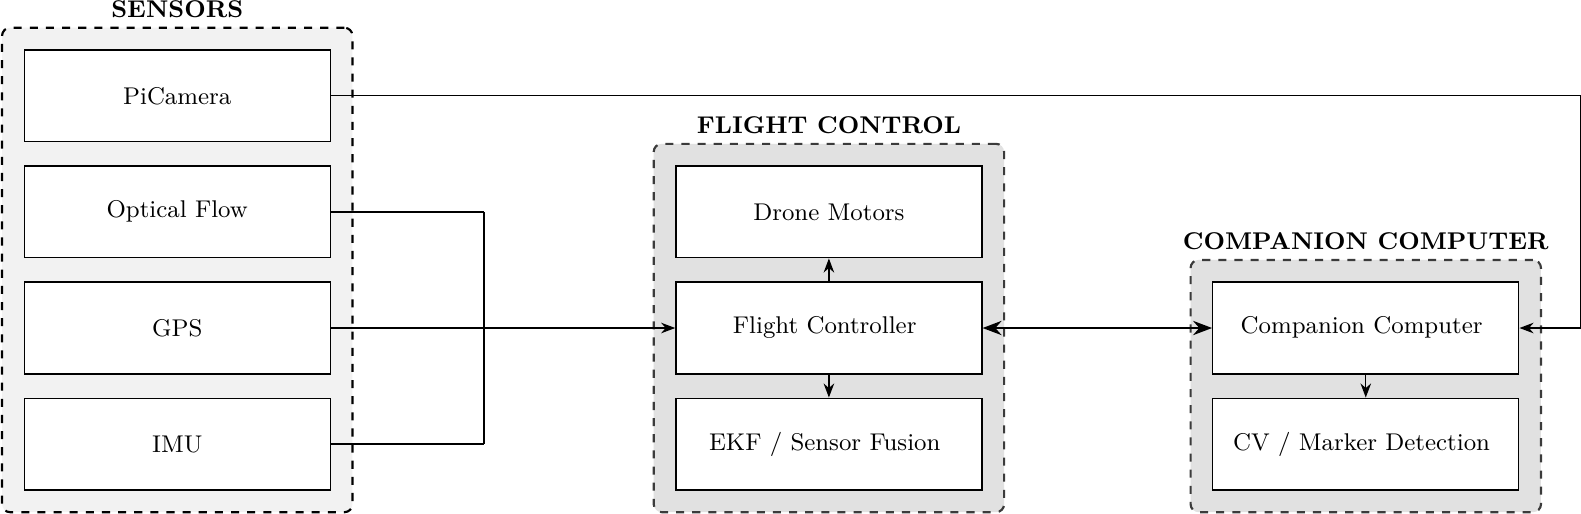
\includegraphics[width=0.7\linewidth]{teams/drone/figures/drone_navigation_dataflow}
    \caption{Drone dataflow and control architecture for autonomous
             navigation and task execution}
    \label{fig:drone_navigation_dataflow}
\end{figure}

\todo[inline]{Add the localization accuracy achieved in testing (e.g.
position error vs ground truth) and example CV detection output -
currently descriptive only, no measured evidence, unlike the rover's
navigational stack.}
